\section{System preparation}
\label{section:dev-sysprep}
\subsection{Installing the hardware}
\label{subsection:dev-sysprep-hardware}
% \textcolor{red}{Acquisition and installation of mCard modules}
\begin{center}
    
\includegraphics[scale=0.7]{img/4-development/multitech-mtac-mfser.png}
    \captionof{figure}{Multi-Tech MTAC-MFSER mCards \citep{multitech-mfser}}
    \label{fig:4-mfser}
\end{center}
The Conduit gateway is shipped by default with the MTAC-LORA accessory card installed. For this project the LoRa capability is not required, so this mCard was removed from the Conduit and replaced with an MTAC-MFSER-DCE card (supplied on loan by Multi-Tech), which provides a female DB9 connector. These cards are easy to install - a single screw holds them in place, and once the screw is removed the card can be removed or installed by sliding it in or out of the Conduit. For the purposes of the project only one mCard was installed and the other slot was covered by a blanking panel, however for production use a second mCard can be installed, allowing the Conduit to provide access to two devices.

\subsection{Updating the Conduit}
\label{subsection:dev-sysprep-updates}
The next stage of development was to ensure that the Conduit gateway was in a good state to work with. Writing software and editing configuration files while the operating system and its packages are out of date may cause issues later on in the project or when used in production, where any updates that are installed can break configurations in a way that is not easily recoverable.\\\\
The Multi-Tech Conduit uses a custom distribution of Linux, although there are similarities between it and Debian. The installed package manager was not one of these similarities, however. Most Debian-based distributions use Aptitude package manager which is managed with the \verb|apt-get| command, but this distribution of Linux uses Opkg package manager, which is managed with the \verb|opkg| command. Aptitude can update the operating system and installed packages by running commands such as \verb|apt-get upgrade|, whereas Opkg can only install and update packages, the install files of which (\verb|.ipk| files) must be passed to Opkg as parameters upon command execution. \\\\
According to \cite{multitech-dev-osupgrade}, upgrading the operating system on the Conduit requires that the upgrade files are placed in a specific directory (\verb|/var/volatile| at the time of writing), then executing the upgrade executable with root privileges. It is recommended that this is done via a console connection to the gateway rather than a remote connection as the upgrade causes the gateway to reboot.

\section{Compiling GNU Screen for ARM}
\label{section:dev-screenonarm}
GNU Screen was chosen as the terminal emulation software that would be used for this project. Installing Screen using the Opkg package manager was impossible as there was no available install package, meaning that the software had to be installed by compiling the binary from the source code. This proved more difficult than normal as, while most desktops and laptops use an x86 architecture, the Conduit is based on an ARM architecture. This required cross-compilation of the source code - that is, an x86-based computer was used to produce an ARM-compatible executable.\\\\
Multi-Tech provides a C/C++ toolchain for Linux-based computers, which aids developers with compiling software for ARM-based processors by automatically setting environment variables, installing dependencies, and installing libraries that are required for the compilation to complete. This requires that compilation takes place on a Linux PC, therefore the compilation was completed on a virtual machine running Ubuntu 19.10. The latest version of the toolchain (5.1.8 at the time of writing) was used to ensure that any potential bugs that had been identified in previous versions were patched, and it was installed by downloading and executing the installation script from the Multi-Tech Developer portal. This script saved the toolchain to \verb|/opt/mlinux/5.1.8/environment-setup-arm926ejste-mlinux-linux-gnueabi|. The command \verb|source .../environment-setup-arm926ejste-mlinux-linux-gnueabi| was added to the \verb|.zshrc| file that executes each time a command line is launched, meaning that the toolchain did not need to be manually activated each time a command line session was started.\\\\
3

\section{Running a second SSH daemon}
\label{section:dev-sshdaemon}
The decision was taken to run a second SSH daemon alongside the pre-existing one specifically for out of band access. Although a second SSH server wasn't required for the system to function, implementing it makes connecting to the managed device easier for the network engineers that need to do so. The alternative to running a secondary daemon is that an engineer must connect normally to the gateway via SSH and manually execute the terminal emulation software. 
\subsection{Creating the second daemon}
\label{subsection:dev-sshdaemon-creating}
In this distribution of Linux, in keeping with older versions of Debian, system services (daemons) are defined within the \verb|/etc/init.d| directory. A default OpenSSH service is installed when the operating system is installed and is defined in the \verb|/etc/init.d/sshd| file. This definition file was duplicated to \verb|/etc/init.d/sshd-oobm| to create a second OpenSSH service specifically for out of band device access, ensuring that as much of the configuration as possible was kept the same to ensure consistency. The service definition file for the out of band service is included in Appendix \ref{section:appendix-sshdoobminitd}.\\\\
To ensure the two SSH daemons acted independently of each other, separate PID files were used. PID files store the process identifier for a given process, which is a unique integer for each running process. Using different PID files should force the default and custom SSH daemons to start under different process IDs and therefore force the custom service to act without reliance on the default service.\\\\
Once the service definition files were created, the configuration files for the custom SSH server were copied from the original files used by the default daemon:
\begin{verbatim}
/
    etc/
        init.d/
            sshd
            sshd-oobm
        ssh/
            sshd_banner
            sshd_config
            sshd_oobm_banner
            sshd_oobm_cmd
            sshd_oobm_config
\end{verbatim}
\captionof{figure}{Filesystem tree of changed files}
\label{fig:4-filetree}
The files in \verb|/etc/init.d| define the services themselves, whereas the files in \verb|/etc/ssh| define the configuration parameters for the service. The location of these files is specified in the service definition file.

\subsection{Configuration}
\label{subsection:dev-sshdaemon-configuration}
The configuration parameters for the second SSH daemon will be kept the same as the original server as much as possible to ensure consistency in their configurations and to prevent crashes.
\subsubsection{Sudoers file}
\label{subsubsection:dev-sshdaemon-configuration-sudoers}
The \verb|/etc/sudoers| file, which controls who can execute commands with root privileges, required editing to allow network administrators to reconfigure the serial card to work in RS-232 mode \citep{multitech-dev-rs232}. The \verb|mts-io-sysfs| command must be executed with root privileges and therefore requires the use of \verb|sudo|. However, it was important that non-administrator users on the gateway were only able to execute that specific command with root privileges, and also that it did not prompt the user for their password. This was accomplished with \verb|%oobm ALL=(ALL:ALL) NOPASSWD: /usr/sbin/mts-io-sysfs|, which specifies that all users in the \verb|oobm| group can become any user, not be asked for their password, and execute only that command.
\subsubsection{Service definition file}
\label{subsubsection:dev-sshdaemon-configuration-initd}
The \verb|/etc/init.d/sshd-oobm| is the service definition file for the \verb|sshd-oobm| service. This file was initially copied from \verb|/etc/init.d/sshd| (the definition file for the standard SSH server), but required some editing to allow the OOBM service to function independently. The PID file that should be used by the service is defined by the variable \verb|PIDFILE| in the service definition. In this instance, the PID file was changed to \verb|/var/run/sshd-oobm.pid|, instead of \verb|/var/run/sshd.pid| which is used by the standard server. The \verb|CONFFILE| variable, which defines where the service should look for its configuration parameters, was also changed to \verb|/etc/ssh/sshd_oobm_config| instead of \verb|/etc/ssh/sshd_config|. The \verb|check_for_no_start| function was modified to check for the existence of \verb|/etc/ssh/sshd_oobm_not_to_be_run| instead of \verb|/etc/ssh/sshd_not_to_be_run|. This function will prevent the server from being started if this file exists. The \verb|check_privsep_dir| function, which checks for the existence of the Privilege Separation home directory, was changed to look for the \verb|/var/run/sshd-oobm| directory as opposed to \verb|/var/run/sshd|. The start, restart, and stop functions were updated to point to OOBM-specific configuration files or PIDs, and the console output (where present) was edited to remind the user that they were changing the behaviour of the OOBM SSH server instead of the standard server. 
\subsubsection{Connection banners}
\label{subsubsection:dev-sshdaemon-configuration-banners}
Two files, \verb|/etc/ssh/sshd_banner| and \verb|/etc/ssh/sshd_oobm_banner|, were created to define connection banners. These banners are presented to the user upon connection and are intended to remind the user which SSH server they have connected to. Figures \ref{fig:4-sshbannerstd} and \ref{fig:4-sshbanneroobm} show the banners in operation.
\begin{center}
    \begin{minipage}{.5\textwidth}
        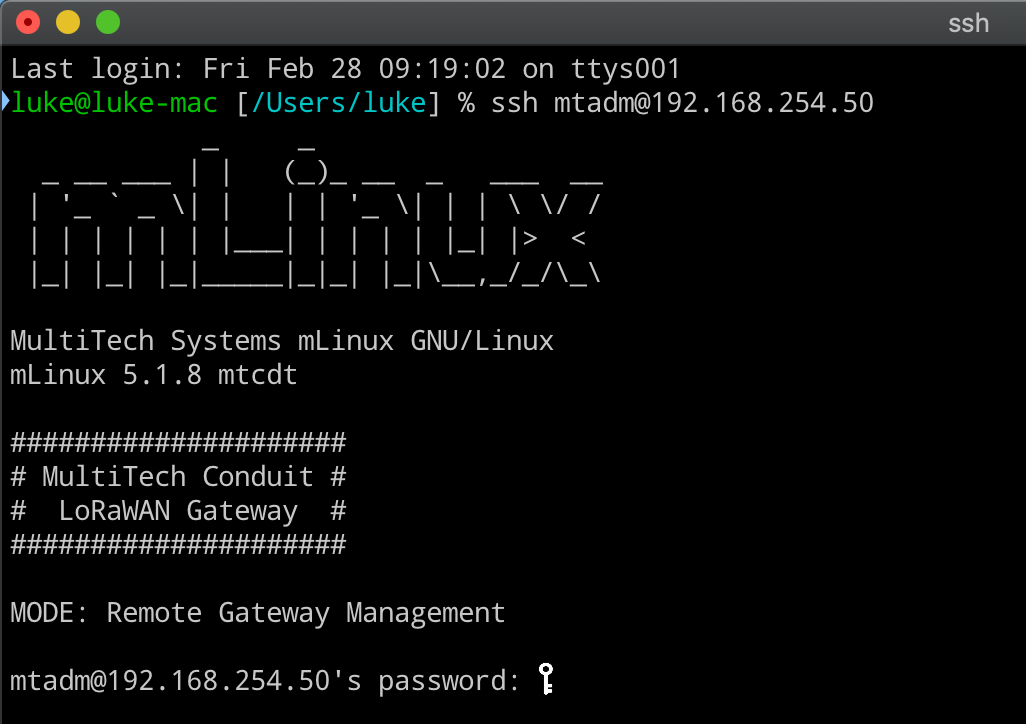
\includegraphics[scale=0.4]{img/4-development/ssh-std-prompt.png}
        \captionof{figure}{Banner: standard server}
        \label{fig:4-sshbannerstd}
    \end{minipage}
    \begin{minipage}{.4\textwidth}
        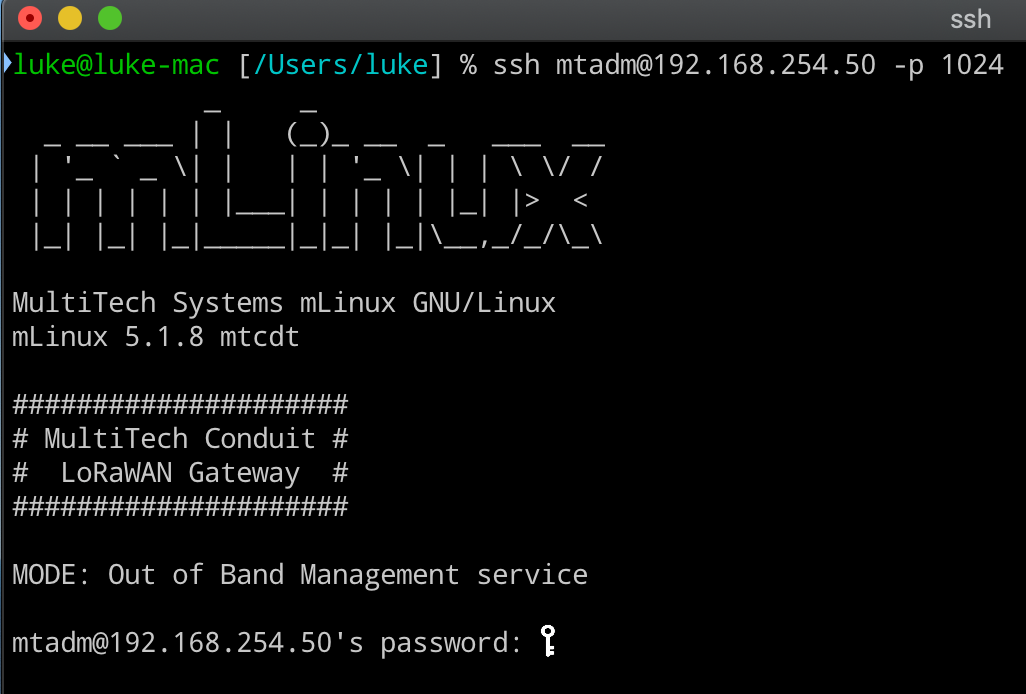
\includegraphics[scale=0.4]{img/4-development/ssh-oobm-prompt.png}
        \captionof{figure}{Banner: OOBM server}
        \label{fig:4-sshbanneroobm}
    \end{minipage}
\end{center}
\subsubsection{Server configuration}
\label{subsubsection:dev-sshdaemon-configuration-sshdoobmconfig}
The configuration parameters for the servers are stored in \verb|/etc/ssh/sshd_config| and \verb|/etc/ssh/sshd_oobm_config|. The \verb|/etc/ssh/sshd_oobm_config| file was created by copying the original file. This helped to save time as all required parameters were already present and only required modification. If starting from scratch, the OpenSSH documentation would have been required to identify the parameters that were required. Many of the parameters in the OOBM configuration were removed as OpenSSH mostly works on the basis that parameters only need to be present if their default value needs to be overridden. \\\\
The \verb|Port| parameter, which controls which TCP port the server listens on, was changed from 22 to 1024, as port 22 is used by the standard SSH server. In a production scenario the chosen port would most likely be changed to a larger number, at least above 10,000. This would help to defend against port scanning attacks which usually associate SSH servers with port 22.\\\\
The Authentication parameters were changed to ensure that authorised users are able to access the connected networking device. A group named \verb|oobm| was created where authorised user accounts can be added. The \verb|AllowGroups| parameter was set to \verb|oobm|, which will ensure that only users in the \verb|oobm| are allowed access to the device. This includes any accounts that have administrative rights on the gateway but are not authorised to access the network device. The \verb|ForceCommand| parameter configures the SSH server to run a command or script upon connection and close the remote connection when the command exits. For the purposes of the OOBM server, this parameter was set to \verb|/etc/ssh/sshd_oobm_cmd| (included in Appendix \ref{section:appendix-ssh-sshdoobmcmd}). This script configures the serial card to operate in RS232 mode, then executes the GNU Screen terminal emulation software. When the user exists GNU Screen, their SSH session is automatically closed.

% \verb|| \verb|| \verb|| \verb||
% \textcolor{red}{See https://github.com/luketainton/oobm-serial for configuration files.}
